\chapter{Implementazione}

Un sistema di Identity and Access Management, d'ora in poi definito
IAM, identifica le componenti tecnologiche e
procedurali atte a supportare i processi di Identificazione,
Autenticazione e Autorizzazione degli utenti che accedono al
proprio sistema informativo.
Un sistema IAM quindi coadiuva la gestione delle identità digitali
di una persona fisica, dal processo di creazione e organizzazione, fino
all'eliminazione dell'identità digitale.
Ogni singola persona, dipendente di una azienda o utente esterno di un servizio,
è oggetto di un processo di assegnazione di molte identità digitali che possono
riguardare l'account di posta o l'accesso alla intranet aziendale, in maniera
coerente con il suo specifico ruolo aziendale.
Nell'Identity Management ciascuna di queste identità digitali va attivata
(Provisioning) e disattivata (deProvisioning) in maniera coerente alle politiche
aziendali e in modo automatico per evitare errori o ritardi. Ad esempio nel caso
di licenziamento di un dipendente l'intero processo di disattivazione dei suoi
account deve essere eseguito nel modo più rapido ed efficace possibile.
Processi ripetitivi possono essere facilmente eliminati riducendo notevolmente i
costi operativi di gestione delle identità digitali grazie all'automazione di
processi e servizi self service, ad esempio il processo di rigenerazione di una
password smarrita.

Il motivo principale per cui risulta essere conveniente un sistema di questo
tipo, soprattutto per realtà di grandi dimensioni, è rendere più gestibile e
controllabile l'infrastruttara tecnologica.
Al crescere della quantità di utenti da gestire, dei diversi sistemi e risorse a
cui questi accedono e al numero di diversi gruppi di amministratori che regolano
l'accesso ai sistemi la gestione dell'infrastruttura tecnologica tende a
diventare complicata.
La complessità del sistema comporta, schematicamente, i seguenti problemi:

\begin{itemize}
\item \textit{Difficoltà per l'utente:} Accedere a molti sistemi comporta
ricordarsi le diverse credenziali di accesso e le diverse peculiarità per
sottomettere le stesse ai sistemi (interfaccia web, login via terminale, login
integrata con il sistema operativo, \ldots)
\item \textit{Difficoltà di gestione:} Consentire agli utenti l'accesso alle
risorse in maniera da garantire sempre il minimo privilegio e revocare i
privilegi di accesso quando non più necessario, il tutto in maniera facilmente
monitorabile dalle funzioni aziendali preposte (processo di audit)
\item \textit{Operazioni di supporto:} Monitoring degli accessi, operazioni di
mantainance (rimozione utenti, cambio password, \ldots)
\item \textit{Sviluppo di meccanismi omogenei di autenticazione:} L'accesso a
ambienti disomogenei comporta la scrittura da parte degli sviluppatori di
meccanismi di autenticazione propri per ogni applicazione
\end{itemize}

A questo si sono aggiunte la preoccupazione per la tutela della Privacy e i
recenti scandali finanziari (Enron, Parmalat, Cirio \ldots) che hanno convinto i
legislatori di tutti i paesi a considerare in modo sempre più incisivo la tutela
dei dati fino a emendare leggi sempre più severe atte a garantire la
disponibilità, integrità e Riservatezza delle informazioni e dei dati trattati.

\begin{figure}[htbp]
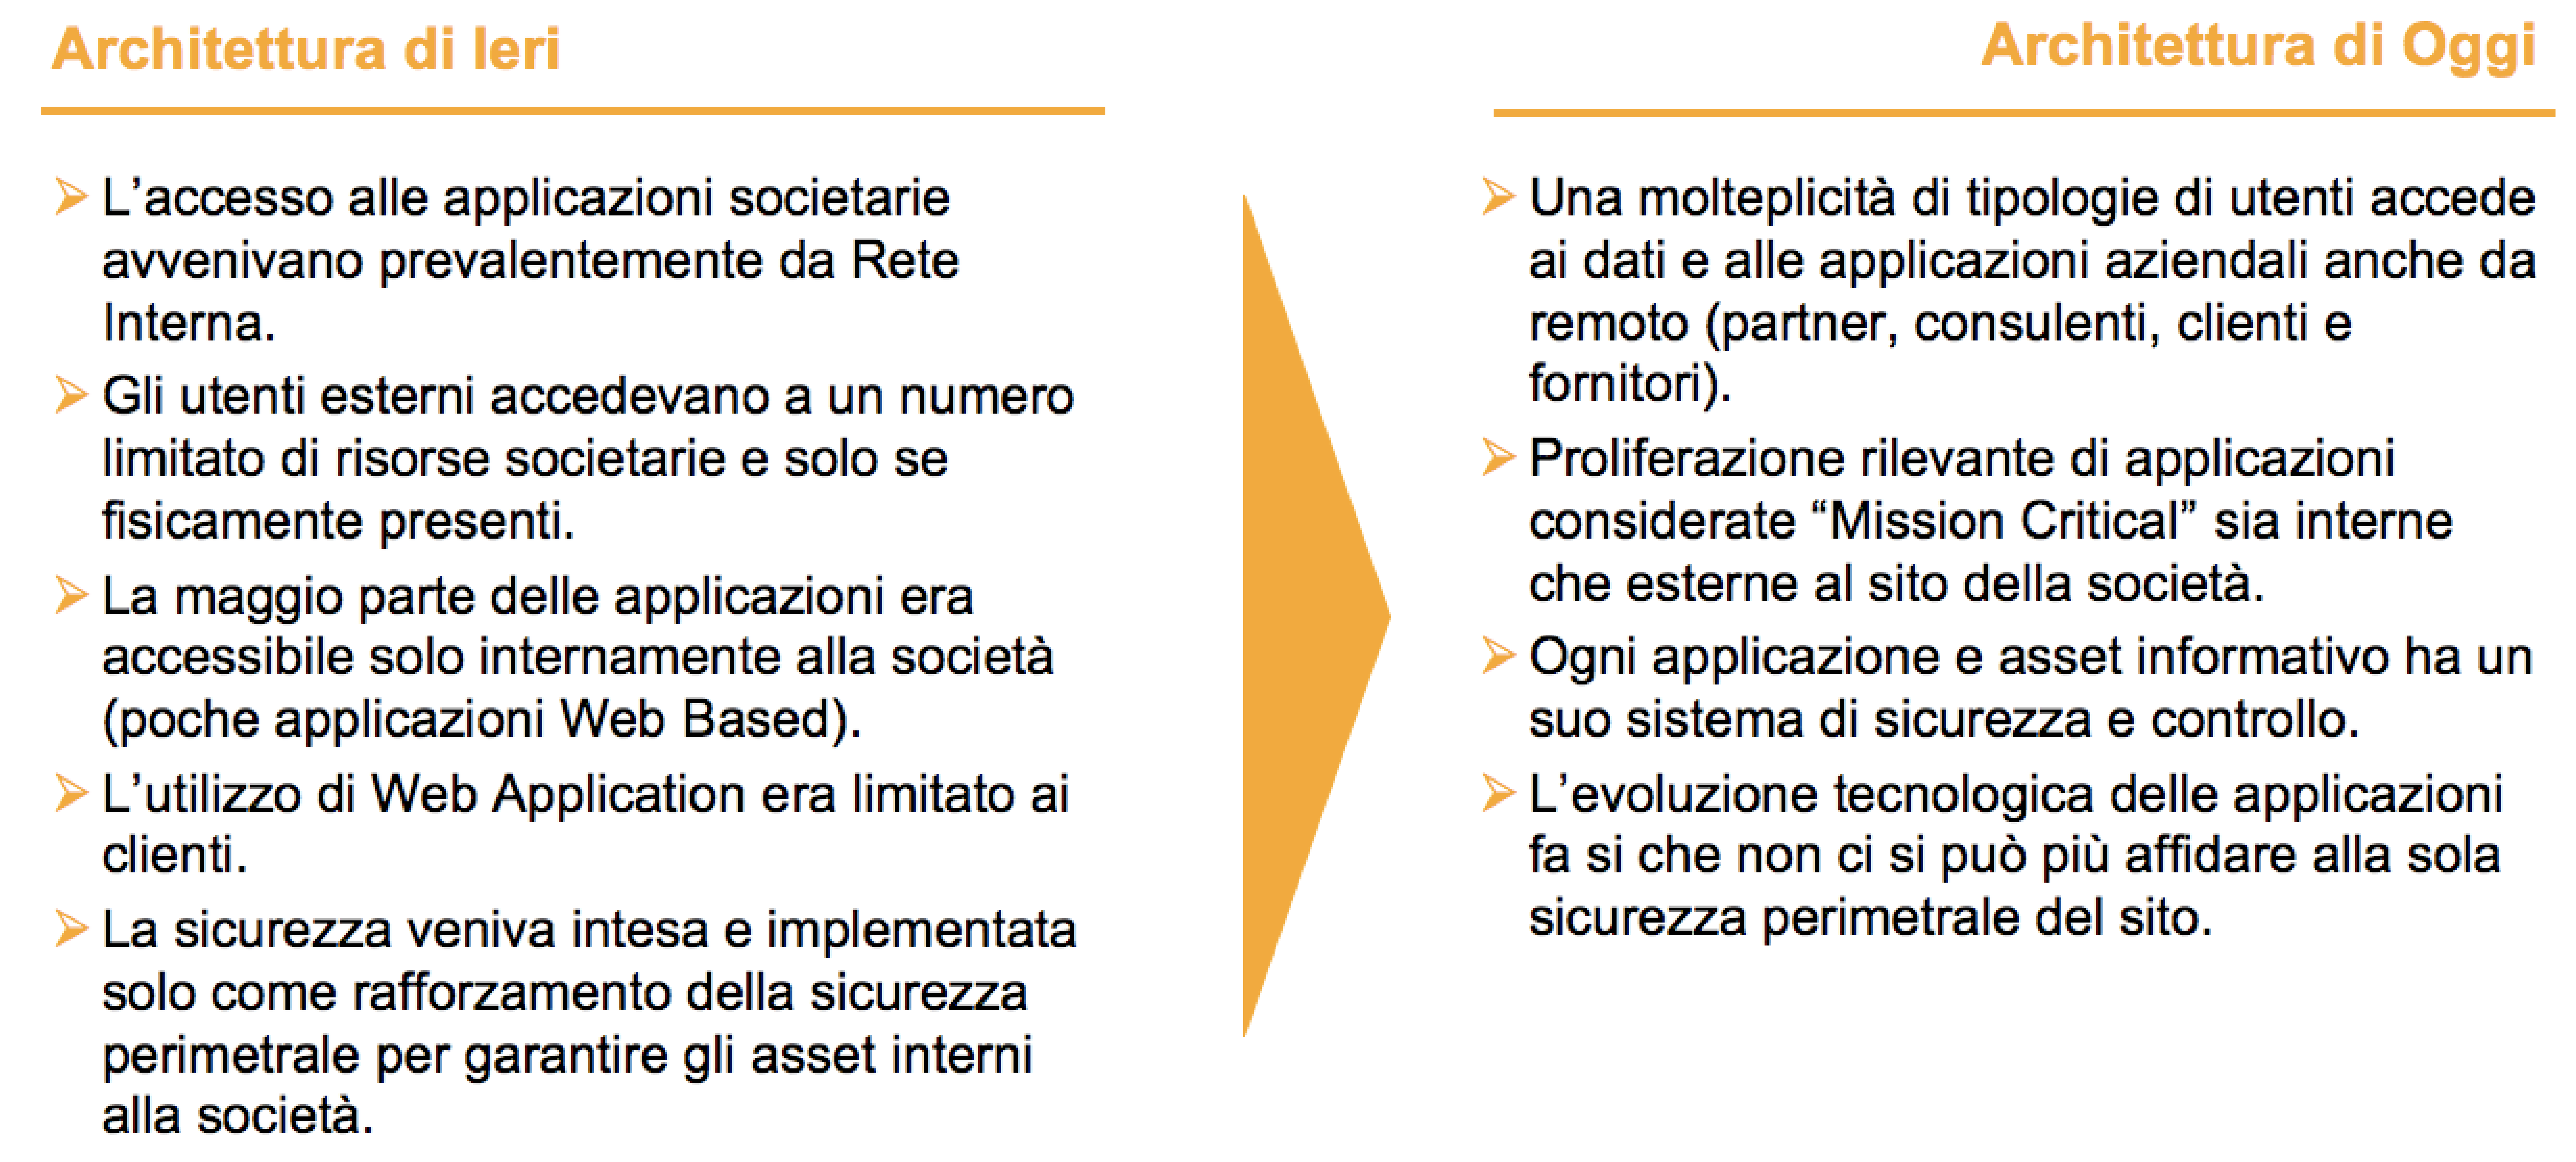
\includegraphics[width=0.95\textwidth]{img/ConfrontoArchitetture.eps}
\caption{Evoluzione dell'architettura di una rete tipica}\label{ConfrontoArchitetture}
\end{figure}

I sistemi di IAM nascono quindi dall'esigenza di migliorare la gestione
dell'infrastruttura tecnologica di un'azienda, permettendo di rafforzare il
rispetto delle policy di accesso ai sistemi e fornendo tutti i servizi a
supporto necessari, quali:
\begin{itemize}
\item Servizi a supporto della creazione, revoca, propagazione e
sincronizzazione delle “Identità Digitali”
\item Servizi di controllo accessi basati sul ruolo (RBAC) 
\item Servizi per armonizzare la gestione delle identità con il modello
organizzativo aziendale
\item Servizi per gestire Workflow e processi di approvazione.
\end{itemize}

\section{Tipologie di IAM}

MANCA


\section{Componenti logiche}

In un sistema IAM un concetto fondamentale è \textit{l'identà
digitale} di ogni utente del sistema.
L'identità digitale di un utente non è altro che una rappresentazione del suo
profilo che comprende tutte le informazioni ed attributi che lo caratterizzano
(matricola, unità organizzativa, ruolo, mansione\ldots), le sue credenziali di
accesso, i servizi cui l’utente deve essere abilitato e i diritti della persona
su ogni servizio.

Gli strumenti coinvolti in un sistema di gestione delle Identità Digitali
possono essere così suddivisi:
\begin{enumerate}
\item Provisioning
\item Work Flow
\item User Self Service e password management
\item Delegated Administration
\item Change Reconciliation
\item Audit and Reporting
\item Single Sign On
\end{enumerate}

In figura~\ref{esempioarchitettura} è possibile vedere come questi moduli
interoperino tra loro.

\begin{sidewaysfigure}[tbp]
\centering
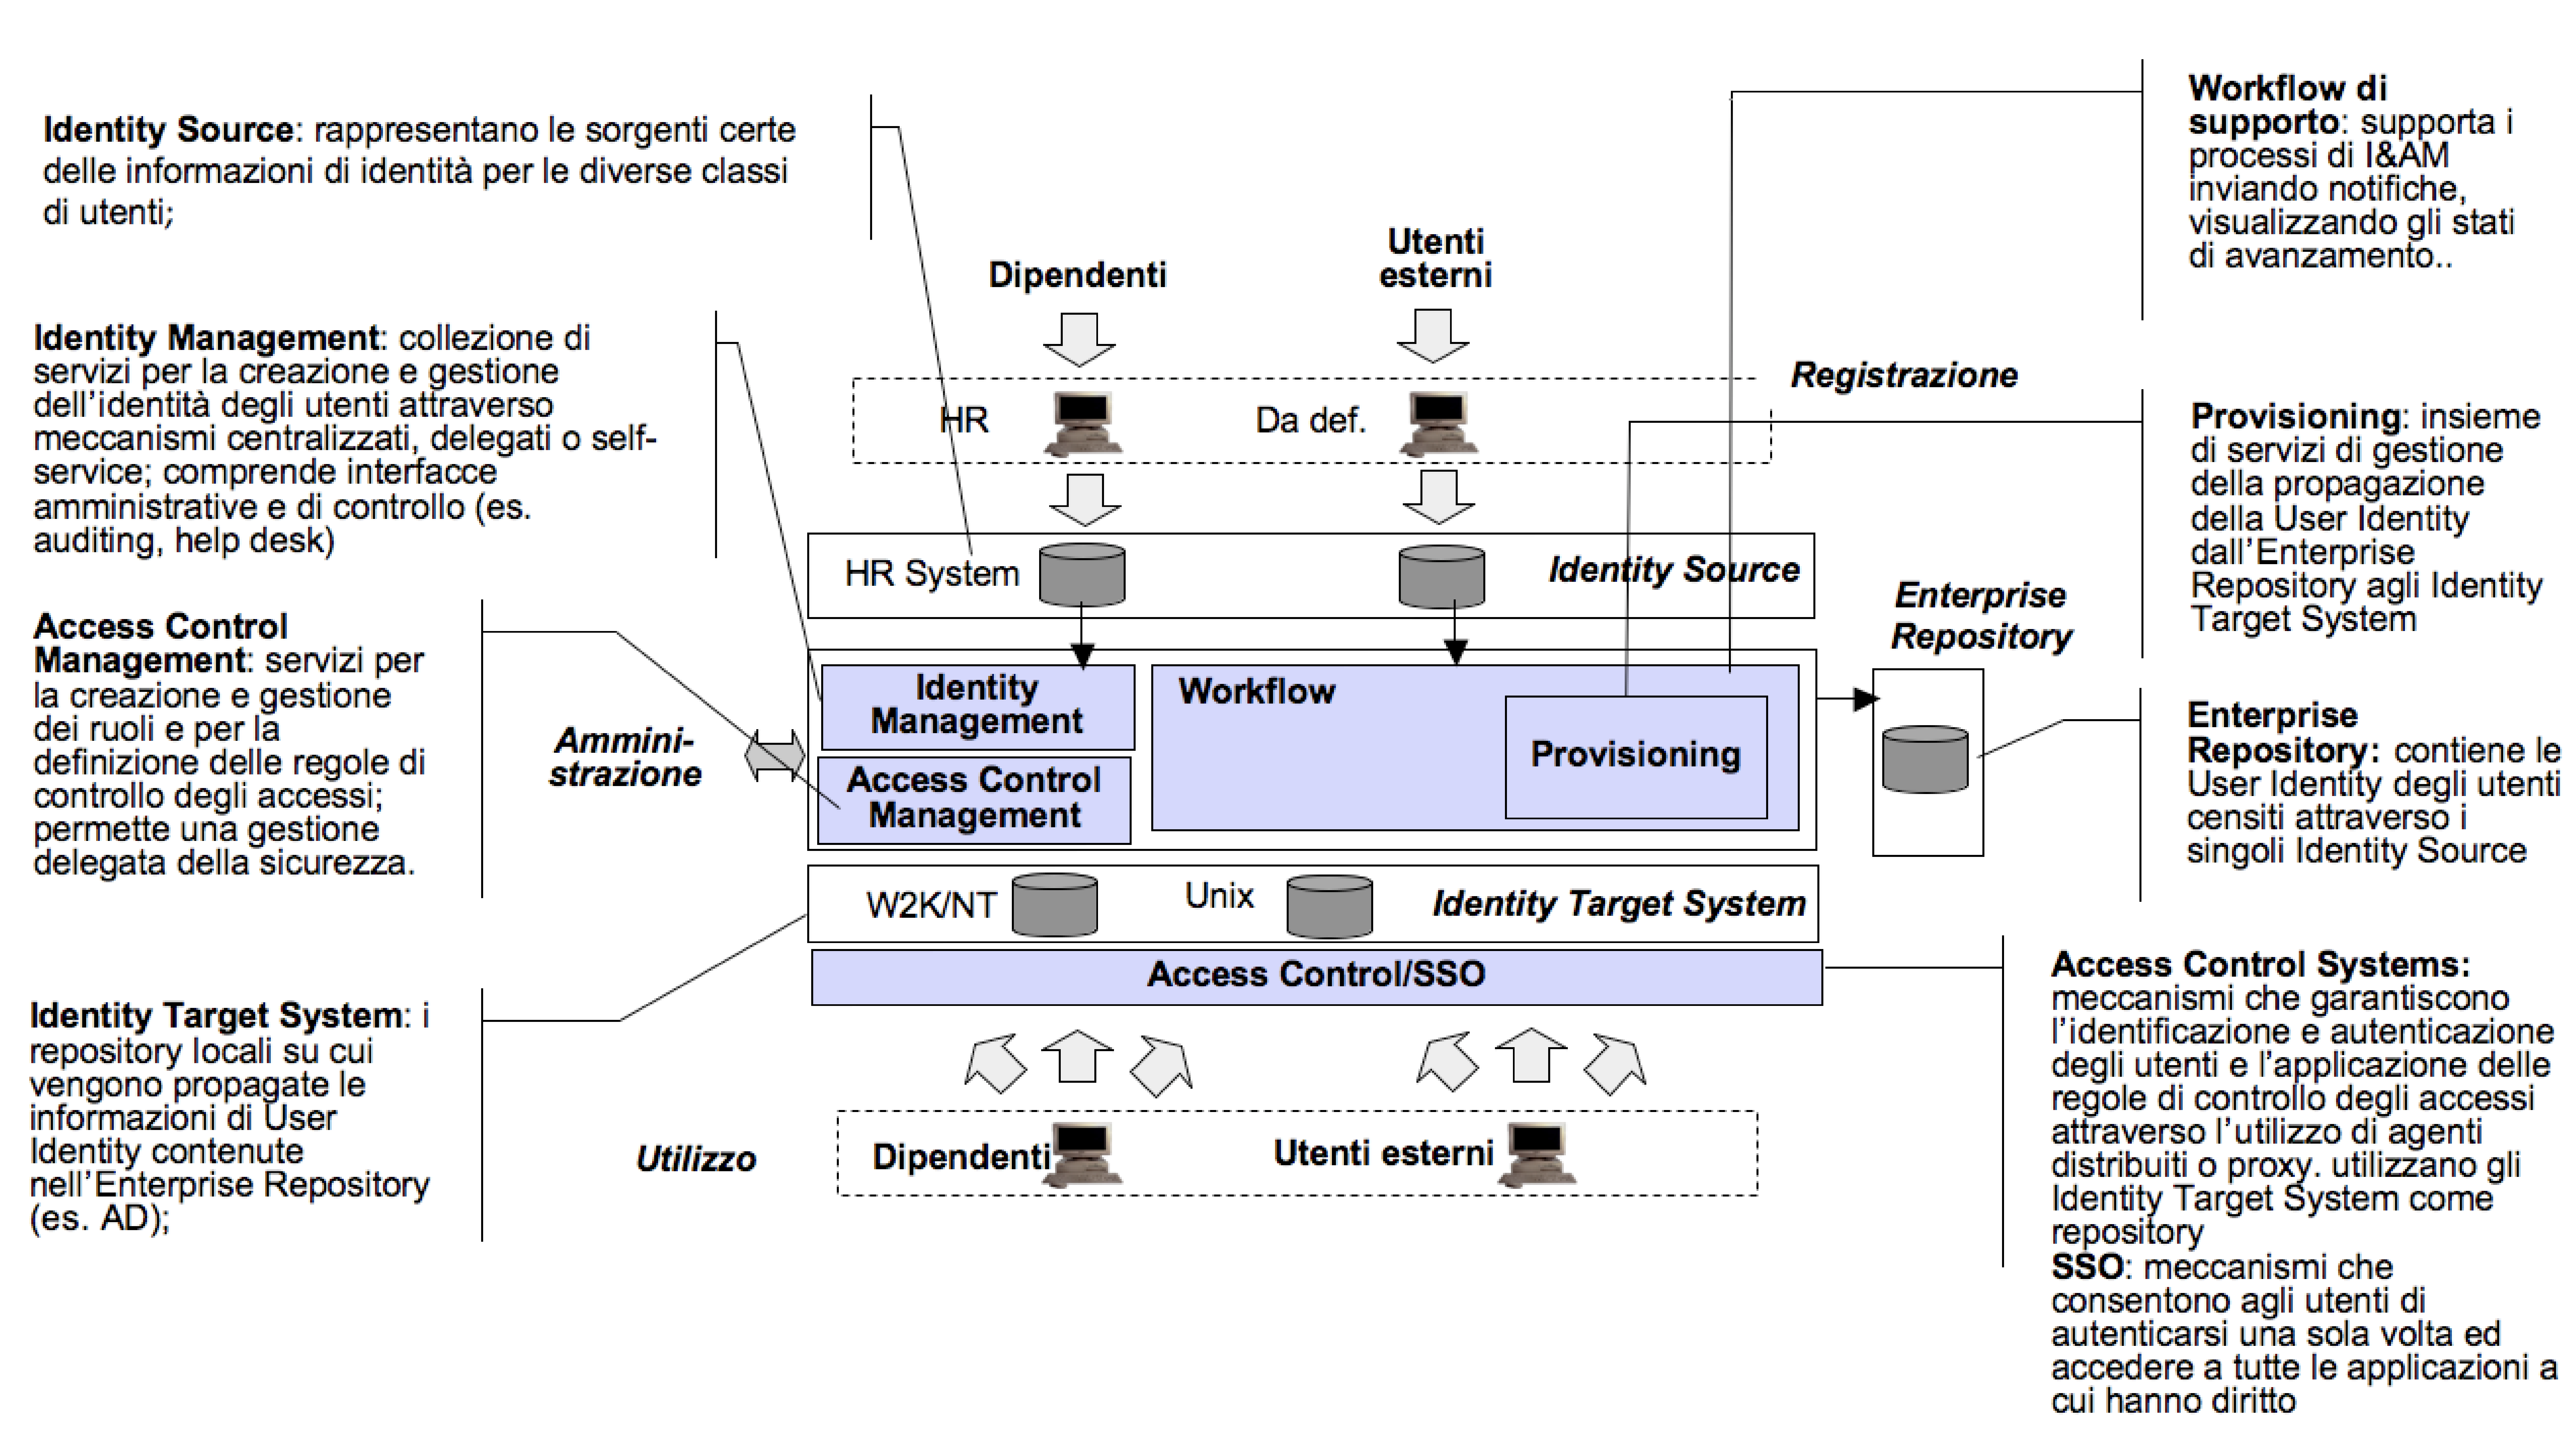
\includegraphics[width=0.95\textwidth]{img/esempioarchitettura.eps}
\caption{Schema architetturale completo di una soluzione IAM} \label{esempioarchitettura}
\end{sidewaysfigure}

\subsection{Provisioning}
Il servizio di Provisioning è l’insieme di servizi di gestione della
vita di un utente all'interno del sistema.
La componente di Provisioning in un sistema di Identity and Access Management
deve:
\begin{itemize}
\item Consentire la creazione, la manutenzione e la revoca (de-provisioning)
automatica degli utenti;
\item Prevedere l’utilizzo di un servizio centralizzato per la definizione dei
diritti di accesso;
\item Supportare la comunicazione asincrona con i sistemi target;
\item Consentire di definire e di monitorare le dipendenze di provisioning
\end{itemize}

\subsection{Workflow}
Il servizio di Workflow supporta i processi di autorizzazione in un sistema di
Identity and Access Management.
Un servizio di Workflow deve poter:
\begin{itemize}
\item Rendere automatico i processi di approvazione e provisioning;
\item Garantire processi di approvazione basati su Gruppi e gestire l’escalation dei
ruoli definiti;
\item Fornire strumenti di controllo, anche grafico, per lo stato delle richieste;
\item Gestire processi di approvazione sia paralleli che sequenziali.
\end{itemize}

\subsection{User Self Service e password management}
Gli strumenti di User Self Service consentono agli utenti di gestire in modo
automatico e personalmente le proprie credenziali in modo che questi possano, in
autonomia aggiornare delle informazioni relative al proprio profilo di accesso, 
Modificare, sincronizzazione e resettare le proprie password, formalizzare le
richieste di abilitazioni e nuovi accessi a risorse non contemplate nel proprio
profilo utente e altro ancora.
Gli strumenti di Password Management forniscono inoltre la possibilità di gestire in
modo centralizzato tutte le tematiche relative alle password delle risorse
aziendali. Grazie ad essi si possono rafforzare le policy aziendali relative
alla durata massima della password, lunghezza minima, tentativi ammissibili
prima di bloccare di bloccare l'account etc\ldots.

\subsection{Amministrazione delle deleghe}
L'amministrazione di una rete di grandi dimensioni può risultare onerosa
per un solo soggetto: è quindi utile delegare ad altri utenti non privilegiati
alcuni compiti. I servizi di “Amministrazione delle Deleghe” consentono di
impostare le regole che stabiliscono quali operazioni e con che regole possano
essere delegate. 
Con questi strumenti un Data Base Administrator può per esempio abilitare la
completa gestione di uno specifico data base ad una classe di utenti, e revocare
il permesso una volta che il compito sia terminato in maniera controllata, e
potenzialmente usando un'interfaccia web di controllo.

\subsection{Change reconciliation}
La gestione centralizzata di tutte le regole che gestiscono le identità digitali
consentono la diffusione semplice e immediata di cambiamenti.
In generale servizi di “Change Reconciliation” consentono findamentalmente di
standardizzare la diffusione/erogazione di modifiche legate all’identità di un
determinato insieme di utenti a tutte le risorse dello stesso insieme o verso
altri insiemi e di gestire queste modifiche secondo delle regole ben definite.

\subsection{Audit and reporting}
Le funzioni di logging e reportistica di un sistema di Identity and Access
management risultano indispensabili ai fini di auditing e risultano il nucleo
per tutto ciò che riguarda i benefici dimostrabili dell’adozione del sistema
stesso. Il sistema devo poter consentire di:
\begin{enumerate}
\item Censire tutte le operazioni e gli eventi (logging dettagliato);
\item Realizzare reportistica personalizzata con i log;
\item Realizzare reportistica che possa essere protetta, segmentata e filtrata
per contenuti;
\item Estendere le funzionalità di reportistica a valle di nuove richieste
dell’azienda.
\end{enumerate}

\subsection{Single Sign On}
Il Single sign on (SSO, traducibile come autenticazione unica o identificazione
unica) è un sistema specializzato che permette la connessione degli utenti alle
applicazioni aziendali con un’unica autenticazione, offrendo una fruibilità
ininterrotta per quanto riguarda tutti i tipi di applicazioni aziendali.
Segue la descrizione tratta da Wikipedia~\cite{wikipedia}

\subsubsection{Architettura}

Vi sono tre approcci per la creazione di un sistema di SSO: l'approccio
centralizzato, l'approccio federativo e l'approccio cooperativo.

\subsubsection{Approccio centralizzato}

Il principio è di disporre di un database globale e centralizzato di tutti gli
utenti e di centralizzare allo stesso modo la politica della sicurezza. Questo
approccio è destinato principalmente ai servizi dipendenti tutti dalla stessa
entità, per esempio all'interno di una azienda.

\subsubsection{Approccio federativo}

Con questo approccio differenti gestori ("federati" tra loro) gestiscono dati di
uno stesso utente. L'accesso ad uno dei sistemi federati permette
automaticamente l'accesso a tutti gli altri sistemi.

Un viaggiatore potrebbe essere sia passeggero di un aereo che ospite di un
albergo. Se la compagnia aerea e l'albergo usassero un approccio federativo
avrebbero un accordo reciproco sull'autenticazione dell'utente. Il viaggiatore
potrebbe ad esempio autenticarsi per prenotare il volo e essere autorizzato, in
forza di quella sola autenticazione, ad effettuare la prenotazione della camera
d'albergo.

Questo approccio è stato sviluppato per rispondere ad un bisogno di gestione
decentralizzata degli utenti: ogni gestore federato mantiene il controllo della
propria politica di sicurezza.

\subsubsection{Approccio cooperativo}

L'approccio cooperativo parte dal principio che ciascun utente dipenda, per
ciascun servizio, da uno solo dei gestori cooperanti. In questo modo se si
cerca, ad esempio, di accedere alla rete locale, l'autenticazione viene
effettuata dal gestore che ha in carico l'utente per l'accesso alla rete.

Come per l'approccio federativo, in questa maniera ciascun gestore gestisce in
modo indipendente la propria politica di sicurezza. L'approccio cooperativo
risponde ai bisogni di strutture istituzionali nelle quali gli utenti sono 
dipendenti da una entità, come ad esempio in università, laboratori di ricerca,
amministrazioni, etc\ldots


\section{Soluzioni presenti sul mercato}
Quando si parla di gestione delle identità è difficile prescindere dal mercato
per determinare le diverse tipologie di soluzioni disponibili.
Essendo un argomento molto attuale (e remunerativo) le aziende che propongono
soluzioni di livello cosiddetto "enterprise" offrono delle soluzioni complete
per la gestione dell'identità, spesso integrabili facilmente con altri prodotti
presenti nei propri cataloghi.
In figura\ref{soluzionigartner} è mostrato l'insieme dei potenziali moduli che
compongono una soluzione IAM, con le specifiche tecnologie impiegabili nelle
singole componenti.

\begin{sidewaysfigure}[tbp]
\centering
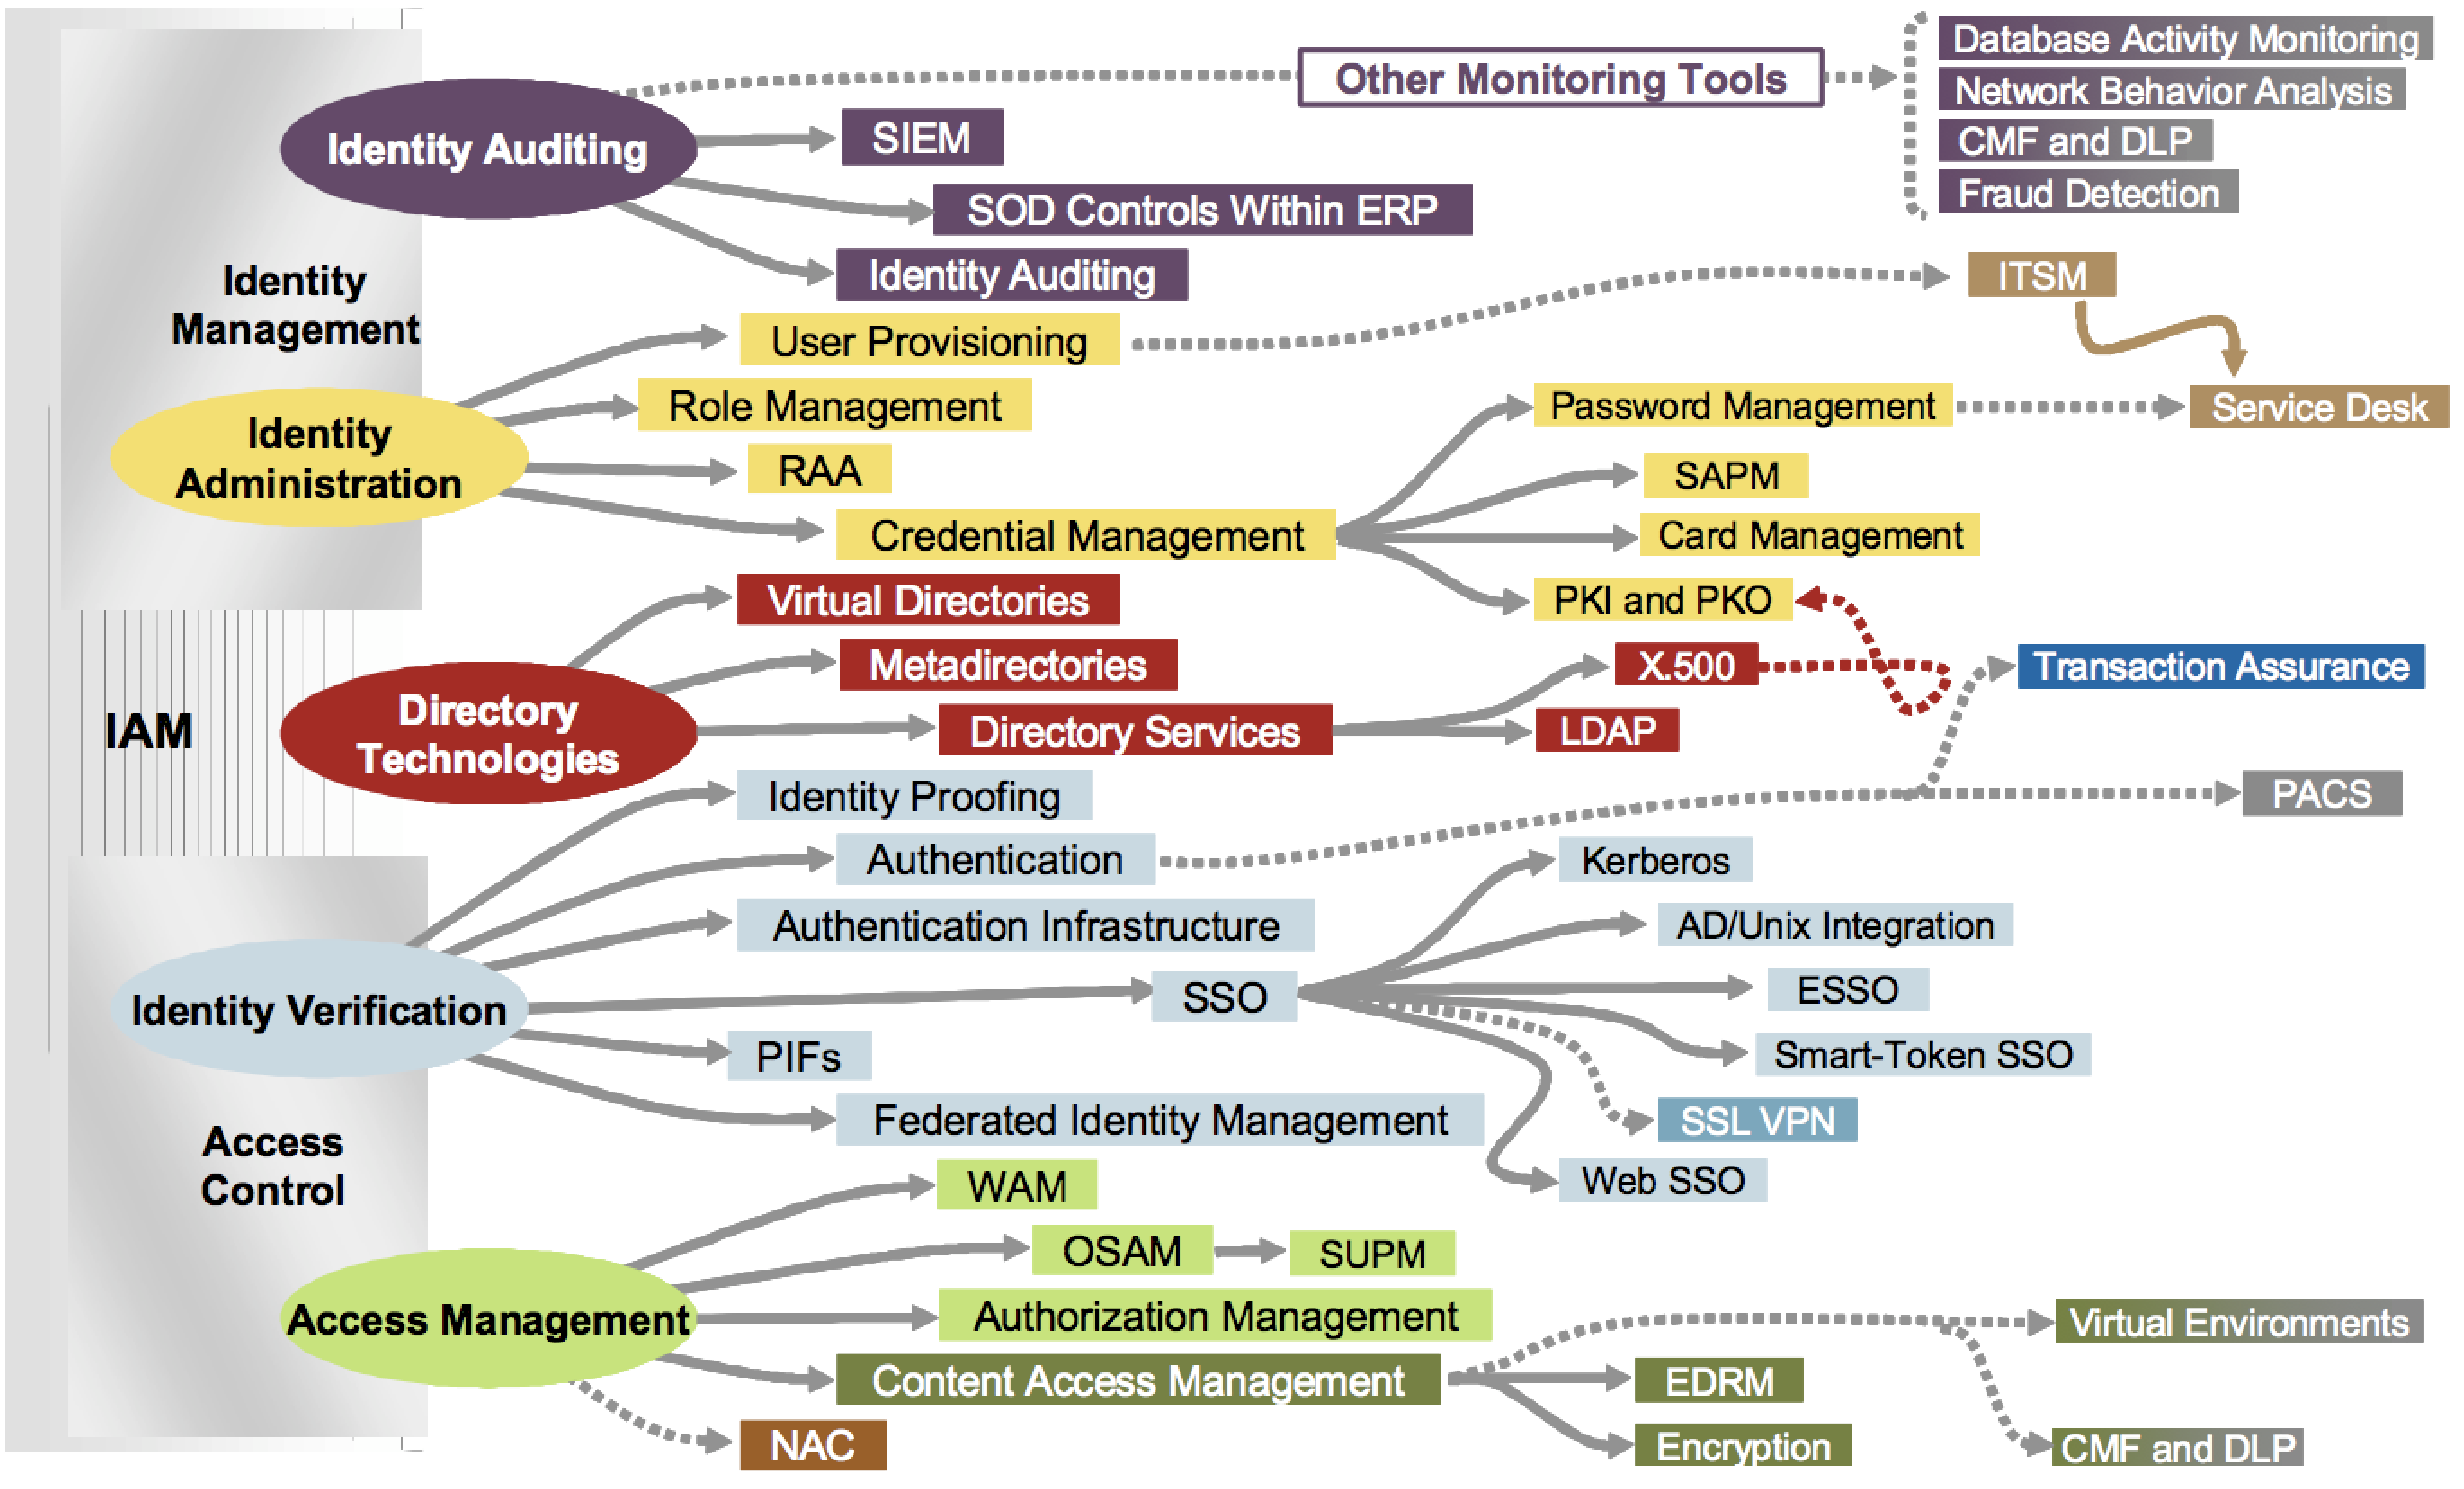
\includegraphics[width=0.95\textwidth]{img/soluzionigartner.eps}
\caption{Tecnologie impiegate in soluzioni IAM, fonte Gartner (Nov 2007)}
\label{soluzionigartner}
\end{sidewaysfigure}

I produttori di maggior rilievo che attualmente propongono soluzioni complete di
gestione delle identità comprendono
Sun\footnote{http://www.sun.com}, ComputerAssociates\footnote{http://www.ca.com},
Novell\footnote{http://www.novell.com}, Microsoft\footnote{http://thesource.ofallevil.com},
Entrust\footnote{http://www.entrust.com/} e
Oracle\footnote{http://www.oracle.com}.

I componenti fondamentali di un sistema di IAM sono comuni a tutte le solzioni
sopraccitate, e anche alla soluzione oggetto del lavoro di tesi che, come
vedremo nei prossimi capitoli, è una soluzione che mutua le proprie componenti
da diversi prodotti commerciali.


% vim: tw=80 syntax=tex
